\documentclass[12pt,spanish,oneside, a4paper]{book}
\usepackage{lmodern}
\usepackage{amssymb,amsmath}
\usepackage{ifxetex,ifluatex}
\usepackage{fixltx2e} % provides \textsubscript
\ifnum 0\ifxetex 1\fi\ifluatex 1\fi=0 % if pdftex
  \usepackage[T1]{fontenc}
  \usepackage[utf8]{inputenc}
\else % if luatex or xelatex
  \ifxetex
    \usepackage{mathspec}
  \else
    \usepackage{fontspec}
  \fi
  \defaultfontfeatures{Ligatures=TeX,Scale=MatchLowercase}
\fi
% use upquote if available, for straight quotes in verbatim environments
\IfFileExists{upquote.sty}{\usepackage{upquote}}{}
% use microtype if available
\IfFileExists{microtype.sty}{%
\usepackage{microtype}
\UseMicrotypeSet[protrusion]{basicmath} % disable protrusion for tt fonts
}{}
\usepackage[inner = 3cm, outer = 2cm, top = 2.5cm, bottom = 2.5cm]{geometry}
\usepackage{hyperref}
\hypersetup{unicode=true,
            pdfauthor={Paola Corrales},
            pdfborder={0 0 0},
            breaklinks=true}
\urlstyle{same}  % don't use monospace font for urls
\ifnum 0\ifxetex 1\fi\ifluatex 1\fi=0 % if pdftex
  \usepackage[shorthands=off,main=spanish]{babel}
\else
  \usepackage{polyglossia}
  \setmainlanguage[]{spanish}
\fi
\usepackage{graphicx,grffile}
\makeatletter
\def\maxwidth{\ifdim\Gin@nat@width>\linewidth\linewidth\else\Gin@nat@width\fi}
\def\maxheight{\ifdim\Gin@nat@height>\textheight\textheight\else\Gin@nat@height\fi}
\makeatother
% Scale images if necessary, so that they will not overflow the page
% margins by default, and it is still possible to overwrite the defaults
% using explicit options in \includegraphics[width, height, ...]{}
\setkeys{Gin}{width=\maxwidth,height=\maxheight,keepaspectratio}
\IfFileExists{parskip.sty}{%
\usepackage{parskip}
}{% else
\setlength{\parindent}{0pt}
\setlength{\parskip}{6pt plus 2pt minus 1pt}
}
\setlength{\emergencystretch}{3em}  % prevent overfull lines
\providecommand{\tightlist}{%
  \setlength{\itemsep}{0pt}\setlength{\parskip}{0pt}}
\setcounter{secnumdepth}{5}
% Redefines (sub)paragraphs to behave more like sections
\ifx\paragraph\undefined\else
\let\oldparagraph\paragraph
\renewcommand{\paragraph}[1]{\oldparagraph{#1}\mbox{}}
\fi
\ifx\subparagraph\undefined\else
\let\oldsubparagraph\subparagraph
\renewcommand{\subparagraph}[1]{\oldsubparagraph{#1}\mbox{}}
\fi

%%% Use protect on footnotes to avoid problems with footnotes in titles
\let\rmarkdownfootnote\footnote%
\def\footnote{\protect\rmarkdownfootnote}

%%% Change title format to be more compact
\usepackage{titling}

% Create subtitle command for use in maketitle
\newcommand{\subtitle}[1]{
  \posttitle{
    \begin{center}\large#1\end{center}
    }
}

\setlength{\droptitle}{-2em}

  \title{}
    \pretitle{\vspace{\droptitle}}
  \posttitle{}
  \subtitle{Validación de parametrizaciones de capa límite utilizando datos de radar}
  \author{Paola Corrales}
    \preauthor{\centering\large\emph}
  \postauthor{\par}
    \date{}
    \predate{}\postdate{}
  
\usepackage{booktabs}
\usepackage{longtable}
\usepackage{array}
\usepackage{multirow}
\usepackage[table]{xcolor}
\usepackage{wrapfig}
\usepackage{float}
\usepackage{colortbl}
\usepackage{pdflscape}
\usepackage{tabu}
\usepackage{threeparttable}
\usepackage{threeparttablex}
\usepackage[normalem]{ulem}
\usepackage{makecell}

\usepackage{setspace}
\setstretch{1.5}
\usepackage{subfig}

\begin{document}

\begin{figure}
\subfloat[Magnitud del viento. \label{caso1-spd}\label{fig:campo-caso11}]{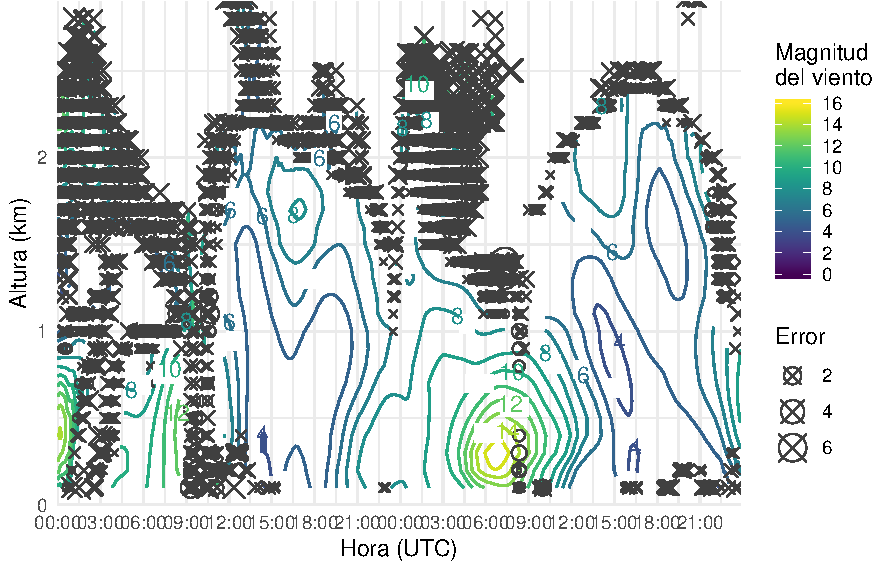
\includegraphics{00_Paper_files/figure-latex/campo-caso1-1} }\newline\subfloat[Dirección. \label{caso1-dir}\label{fig:campo-caso12}]{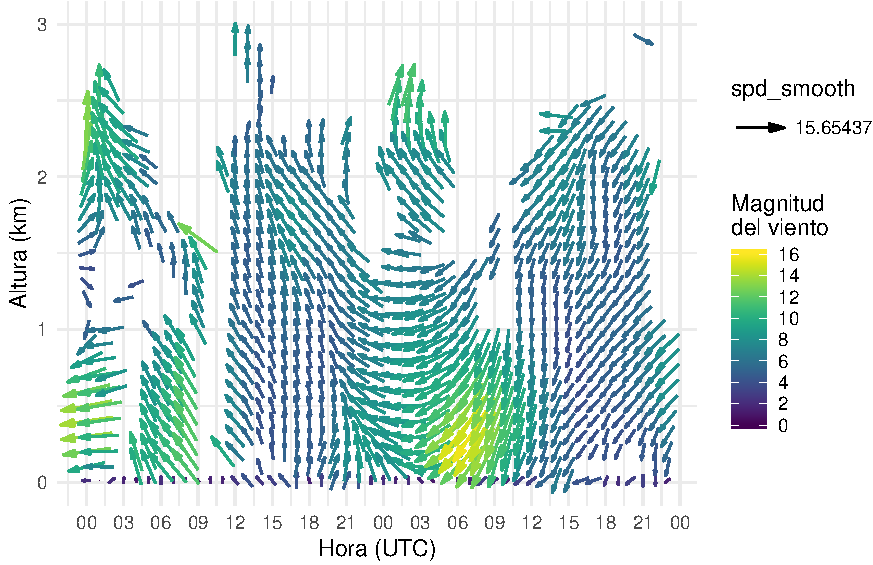
\includegraphics{00_Paper_files/figure-latex/campo-caso1-2} }\caption{Intensidad (m/s) y dirección del viento (grados) correspondiente al Caso 1 (14/01/2016) estimados a partir de las observaciones de radar utilizando la técnica VAD. En el caso de la magnitud del viento se muestran los errores calculados ($dispersi\acute{o}n$ en círculos y $rmse$ en cruces) cuando superan los 0.5 m/s. \label{campo-caso1}}\label{fig:campo-caso1}
\end{figure}

\begin{figure}

{\centering 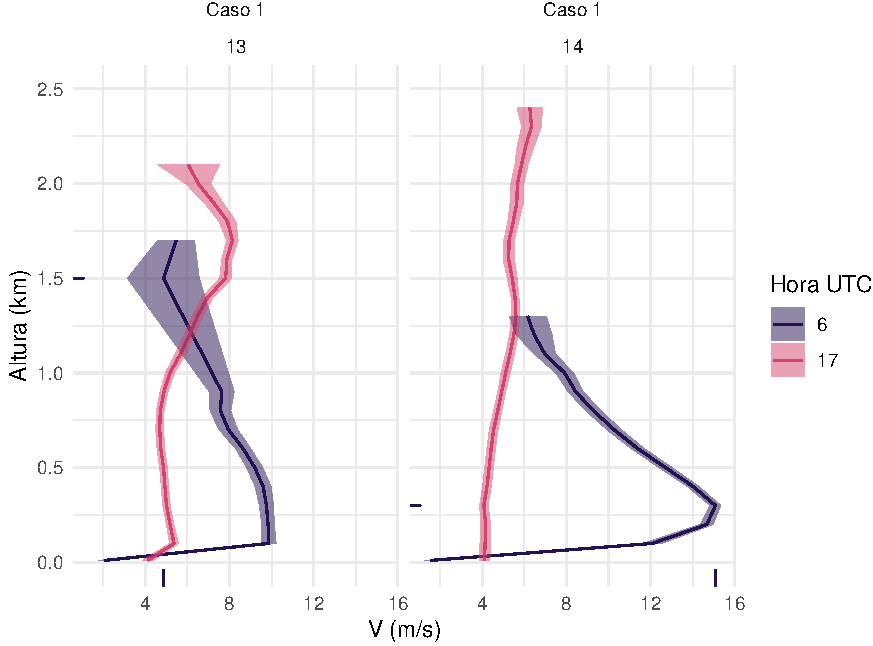
\includegraphics{00_Paper_files/figure-latex/perfiles-1} 

}

\caption{Perfil vertical de viento (m/s) estimado a partir de los datos de radar a las 06 y las 17 UTC y el $rmse$ (m/s) en cada punto (sombreado) para los tres casos. Las marcas en los ejes indican la magnitud del viento máxima y mínima (por encima del LLJ) y la altura a la que ocurren. Los valores en superficie fueron obtenidos a partir de los datos del la estación meteorológica Paraná Aero. \label{perfiles-horarios}}\label{fig:perfiles}
\end{figure}

\begin{figure}

{\centering 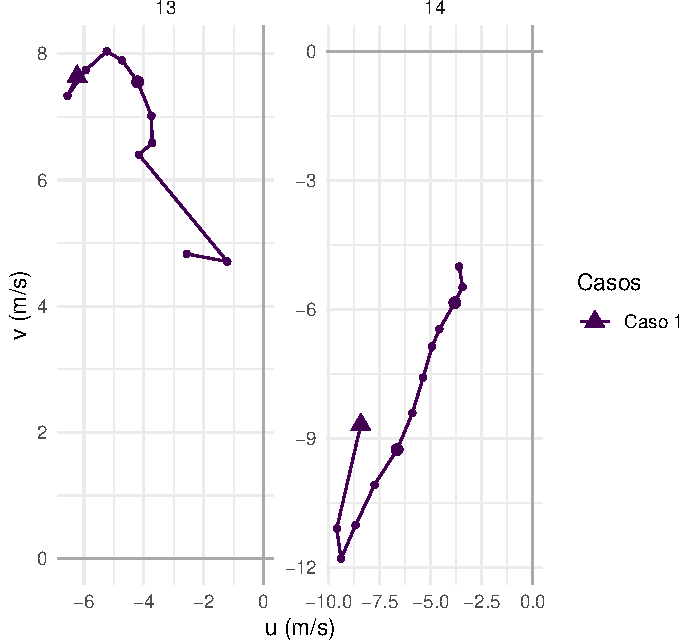
\includegraphics{00_Paper_files/figure-latex/hodografa-horaria-1} 

}

\caption{Hodógrafa en función de la altura entre 100 y 3000 metros, para cada caso de estudio observada por el radar a las 06 UTC. El triángulo marca el nivel inferior y los círculos grandes se ubican cada 500 metros. \label{hodografa-h}}\label{fig:hodografa-horaria}
\end{figure}

\begin{figure}

{\centering \subfloat[Datos observados en la estación meteorológica. \label{hodo-nivel1}\label{fig:hodografa-nivel1}]{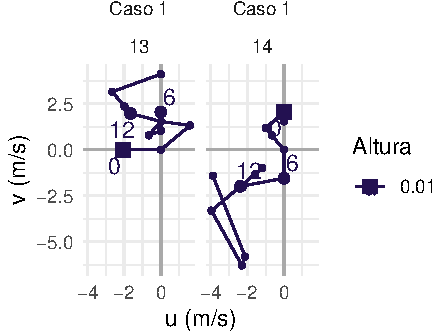
\includegraphics{00_Paper_files/figure-latex/hodografa-nivel-1} }\newline\subfloat[Datos observados por el radar. \label{hodo-nivel2}\label{fig:hodografa-nivel2}]{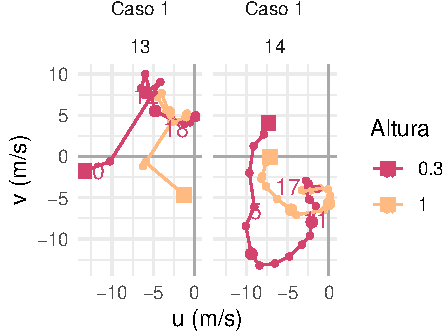
\includegraphics{00_Paper_files/figure-latex/hodografa-nivel-2} }

}

\caption{Hodógrafa temporal para el nivel correspondiente a los datos de la estación meteorológica (a) y 0.3 y 1 km a partir de la estimación del viento con los dato del radar (b). el cuadrado marca el primer tiempo (00 UTC) y cada círculo representa un valor horario (con circulos más grandes cada 6 horas). \label{hodografa-n}}\label{fig:hodografa-nivel}
\end{figure}

\begin{figure}

{\centering 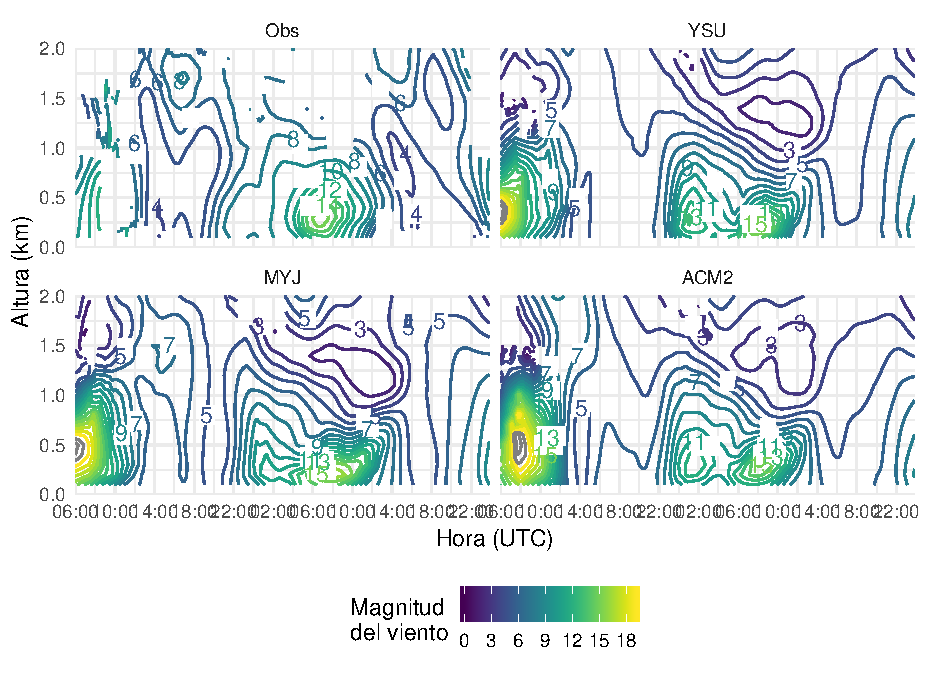
\includegraphics{00_Paper_files/figure-latex/vad-modelo-spd-1} 

}

\caption{Magnitud del viento (m/s) estimada a partir de los datos de radar (Obs) y simulada por el modelo WRF utilizando distintos esquemas de CLP para el Caso 1 (14/01/2016) y posteriormente procesados con la técnica VAD. \label{modelo-spd}}\label{fig:vad-modelo-spd}
\end{figure}

\begin{figure}

{\centering 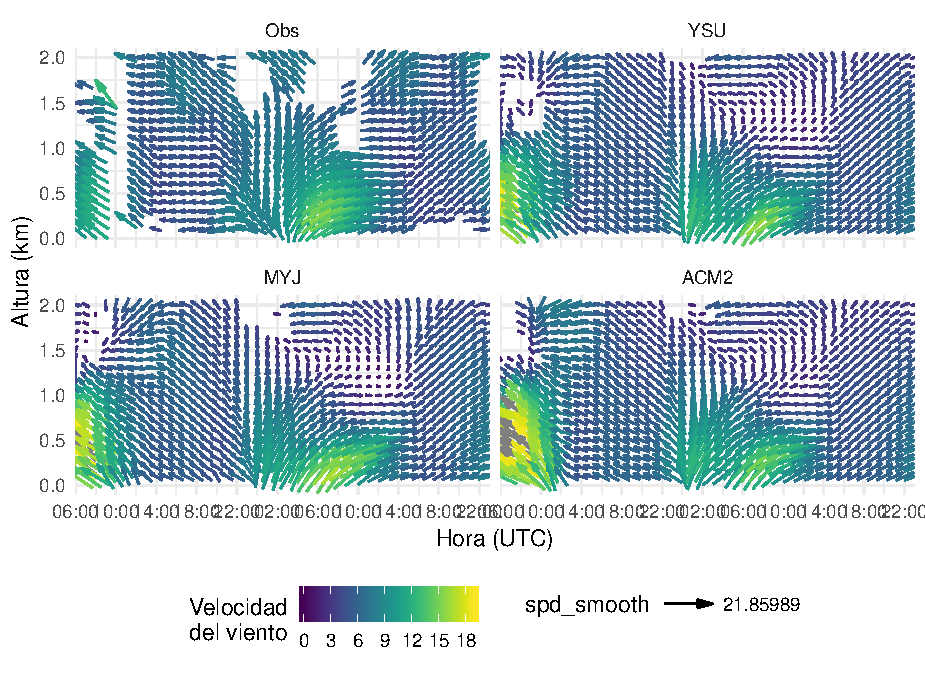
\includegraphics{00_Paper_files/figure-latex/vad-modelo-dir-1} 

}

\caption{Dirección del viento (grados) estimada por el radar (Obs) y simulada por el modelo WRF utilizando distintos esquemas de CLP para el Caso 1 (14/01/2016) y posteriormente procesados con VAD. \label{modelo-dir}}\label{fig:vad-modelo-dir}
\end{figure}

\begin{figure}
\subfloat[Magnitud del viento (m/s) \label{dif-spd}\label{fig:diferencia1}]{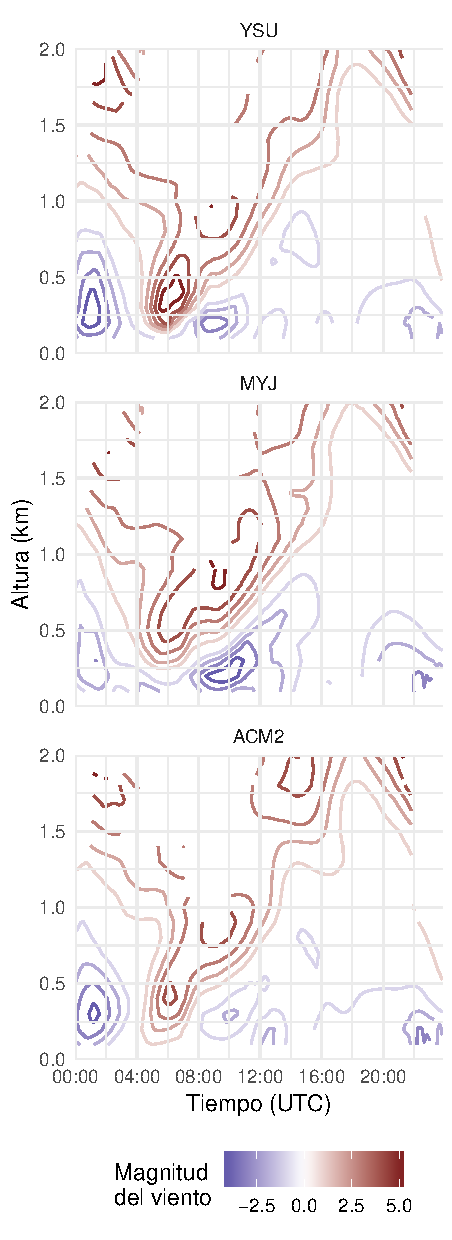
\includegraphics{00_Paper_files/figure-latex/diferencia-1} }\subfloat[Ángulo de la dirección del viento (grados) \label{dif-dir}\label{fig:diferencia2}]{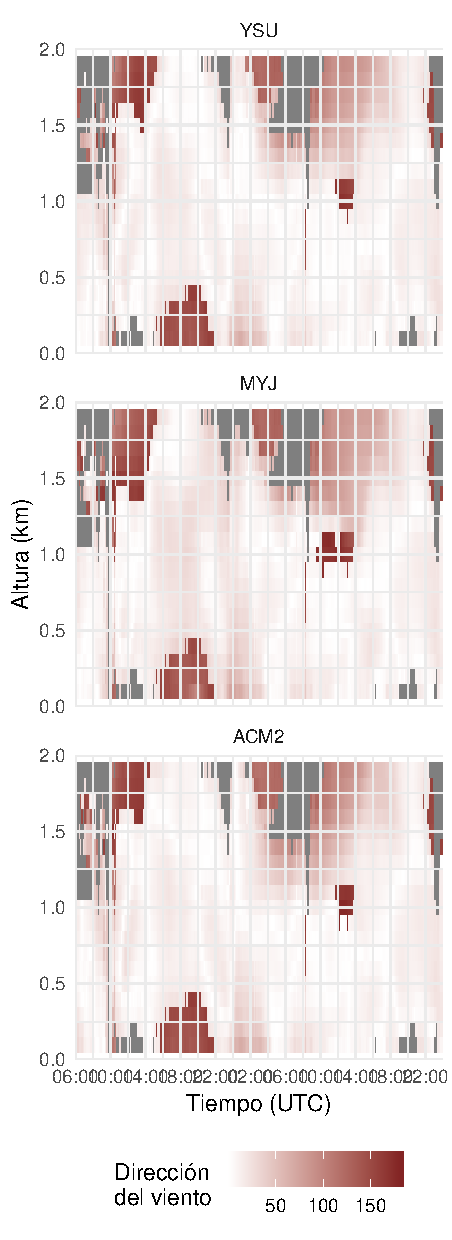
\includegraphics{00_Paper_files/figure-latex/diferencia-2} }\caption{Diferencia entre las observaciones y cada simulación para la magnitud del viento (m/s) (a) y el ángulo de la dirección del viento (grados) (b) correspondiente al Caso 1. \label{dif}}\label{fig:diferencia}
\end{figure}

\begin{figure}
\centering
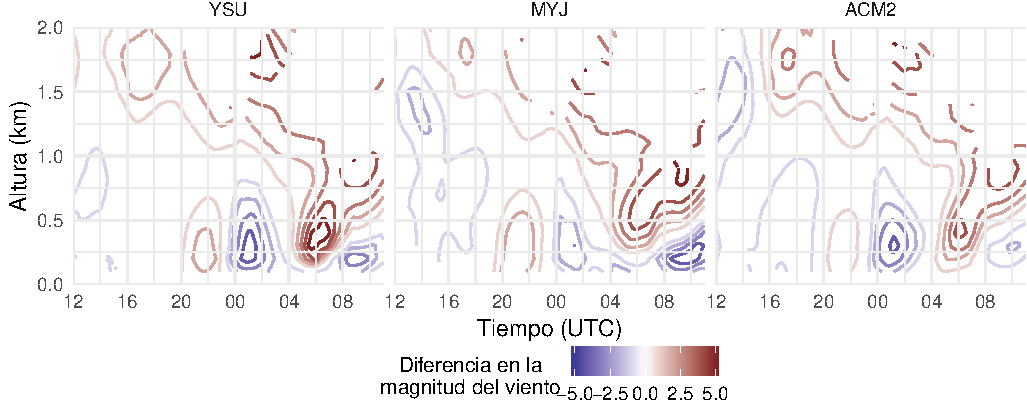
\includegraphics{00_Paper_files/figure-latex/diff_spd-1.pdf}
\caption{Diferencia entre las observaciones y cada simulación para la
magnitud del viento (m/s) correspondiente al Caso 1. \label{dif}}
\end{figure}

\begin{figure}

{\centering 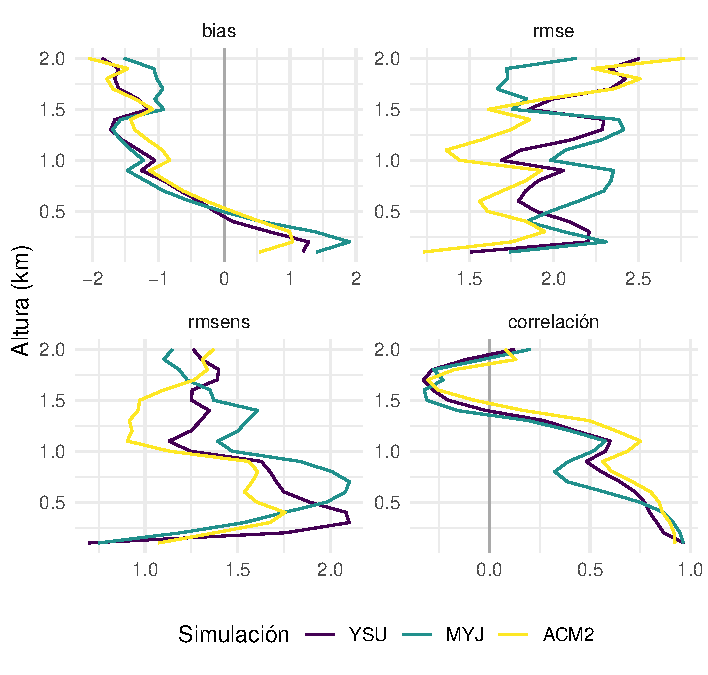
\includegraphics{00_Paper_files/figure-latex/err-spd-1} 

}

\caption{Bias, rmse y rmsens en m/s y coeficiente de correlación para la estimación de la velocidad del viento (m/s) con cada simulación en función de la altura y la simulación. \label{err-spd}}\label{fig:err-spd}
\end{figure}

\begin{table}

\caption{\label{tab:err-tabla}Comparación entre las simulaciones y las observaciones de radar a partir de distintos errores. El bias, rmse, rmsens se expresan en m/s. \label{err}}
\centering
\begin{tabular}[t]{lrrrrrrrr}
\toprule
\multicolumn{1}{c}{ } & \multicolumn{4}{c}{Velocidad} & \multicolumn{4}{c}{Dirección} \\
\cmidrule(l{2pt}r{2pt}){2-5} \cmidrule(l{2pt}r{2pt}){6-9}
caso & bias & rmse & rmsens & correlación & bias & rmse & rmsens & correlación\\
\midrule
YSU & -0.826 & 2.073 & 1.867 & 0.713 & -11.980 & 31.347 & 28.747 & 0.608\\
MYJ & -0.645 & 2.067 & 1.942 & 0.708 & -14.564 & 47.055 & 44.510 & 0.522\\
ACM2 & -0.739 & 1.878 & 1.695 & 0.753 & -13.174 & 33.620 & 30.677 & 0.622\\
\bottomrule
\end{tabular}
\end{table}

\begin{figure}

{\centering 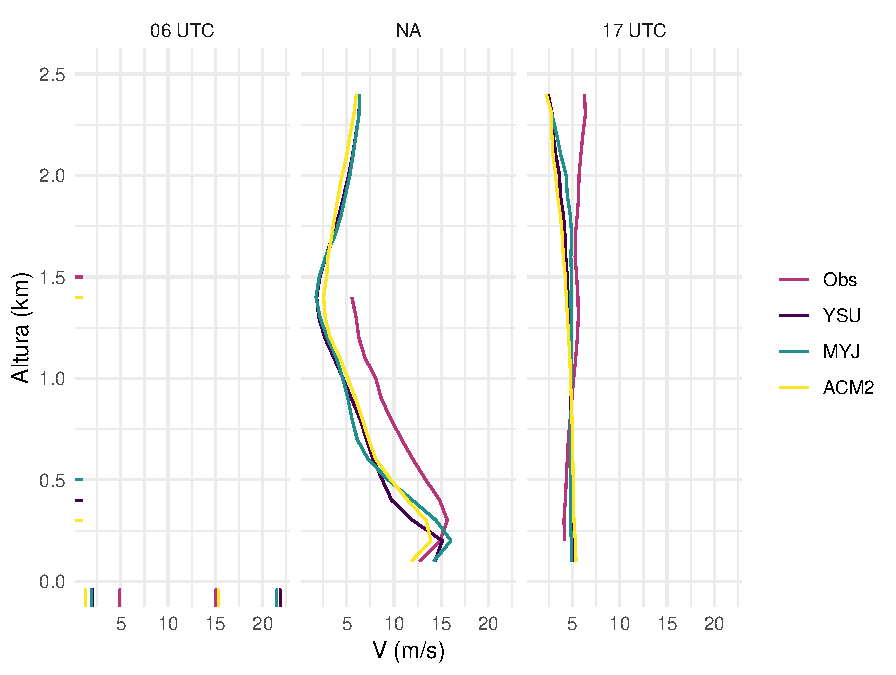
\includegraphics{00_Paper_files/figure-latex/perfiles-mod-1} 

}

\caption{Perfil de viento (m/s) observado por el radar a las 06 y las 17 UTC y perfiles simulados por el modelo para los mismos momentos. Las marcas en los ejes indican la magnitud del viento máxima y mínima y la altura a la que ocurren. \label{perfil-mod}}\label{fig:perfiles-mod}
\end{figure}

\begin{figure}

{\centering 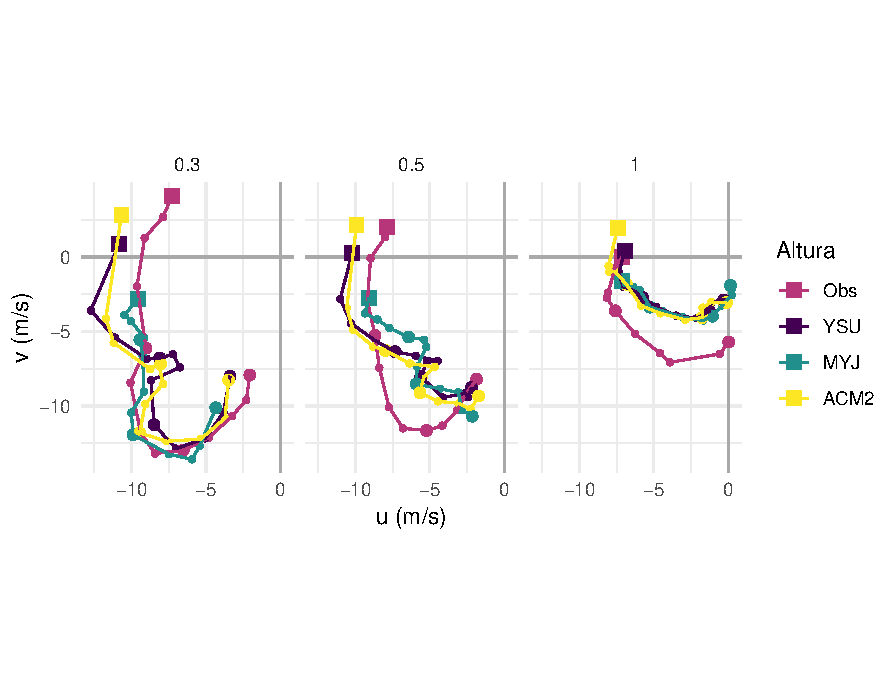
\includegraphics{00_Paper_files/figure-latex/hodografa-wrf-1} 

}

\caption{Hodógrafa temporal para tres niveles. Cada círculo representa un valor horario (con circulos más grandes cada 4 horas) y el cuadrado marca el primer tiempo (00 UTC). \label{hodografa-mod}}\label{fig:hodografa-wrf}
\end{figure}

\begin{figure}

{\centering 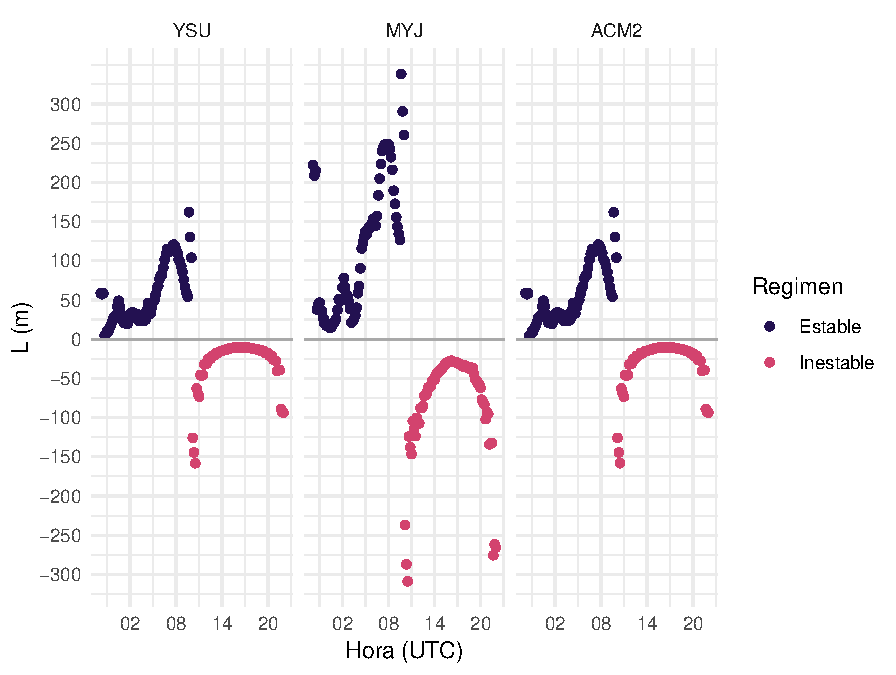
\includegraphics{00_Paper_files/figure-latex/L-parm-1} 

}

\caption{Longitud de Monin Obukhov (m) en función del tiempo, para cada simulación. Los puntos violetas corresponden al régimen estable (nocturno) y los puntos rosas corresponden al régimen inestable (diurno) \label{L-param}}\label{fig:L-parm}
\end{figure}

\begin{figure}

{\centering \subfloat[Estimada directamente por cada esquema de CLP. \label{pblh}\label{fig:pblh-wrf1}]{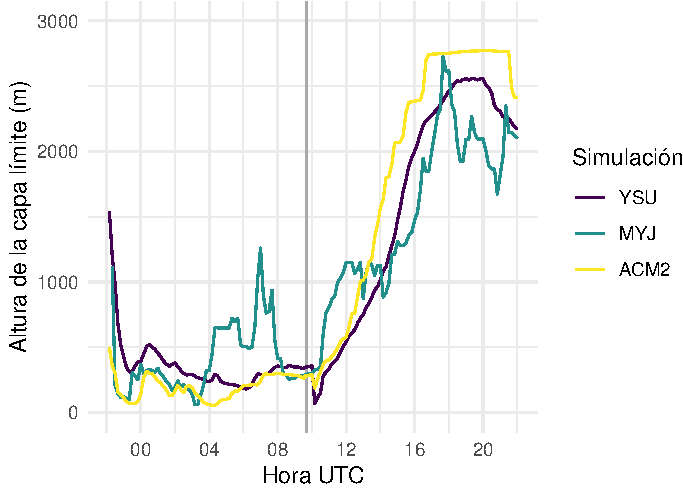
\includegraphics{00_Paper_files/figure-latex/pblh-wrf-1} }\newline\subfloat[Comparación entre la altura calculada por cada esquema (línea) y la estimada a partir de la altura del viento máximo (puntos) sólo en el período estable. \label{pblh-spd}\label{fig:pblh-wrf2}]{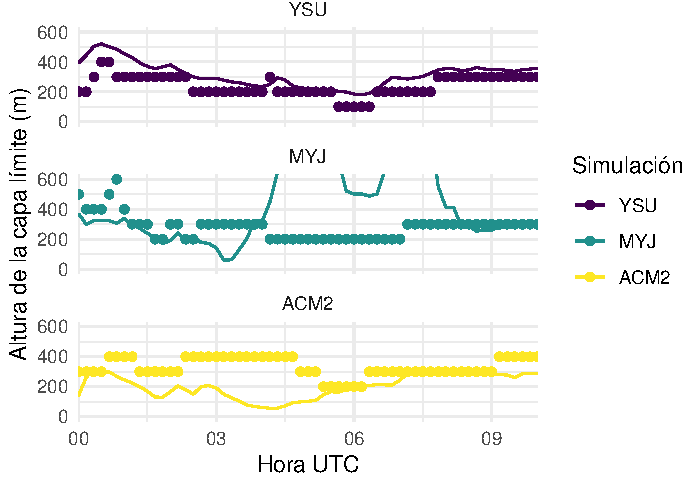
\includegraphics{00_Paper_files/figure-latex/pblh-wrf-2} }

}

\caption{Altura de la capa límite (m) en cada simulación. \label{pblh-wrf}}\label{fig:pblh-wrf}
\end{figure}

\begin{figure}

{\centering 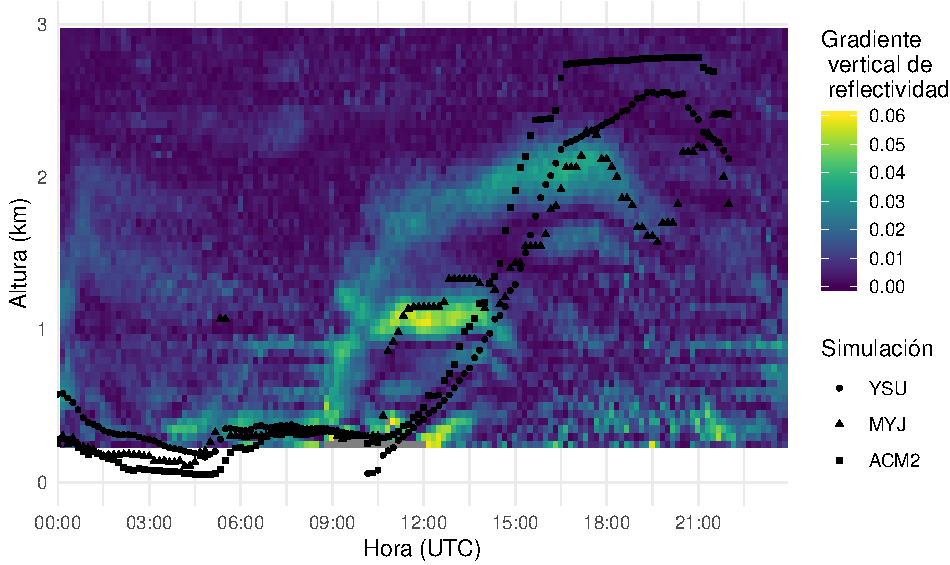
\includegraphics{00_Paper_files/figure-latex/dbz-wrf-1} 

}

\caption{Valor absoluto del gradiente vertical de reflectividad (dBZ/m) en función de la altura y el tiempo para el Caso 1 y la altura de la capa límite estimada en cada simulación. \label{dbz-wrf}}\label{fig:dbz-wrf}
\end{figure}

\begin{figure}

{\centering 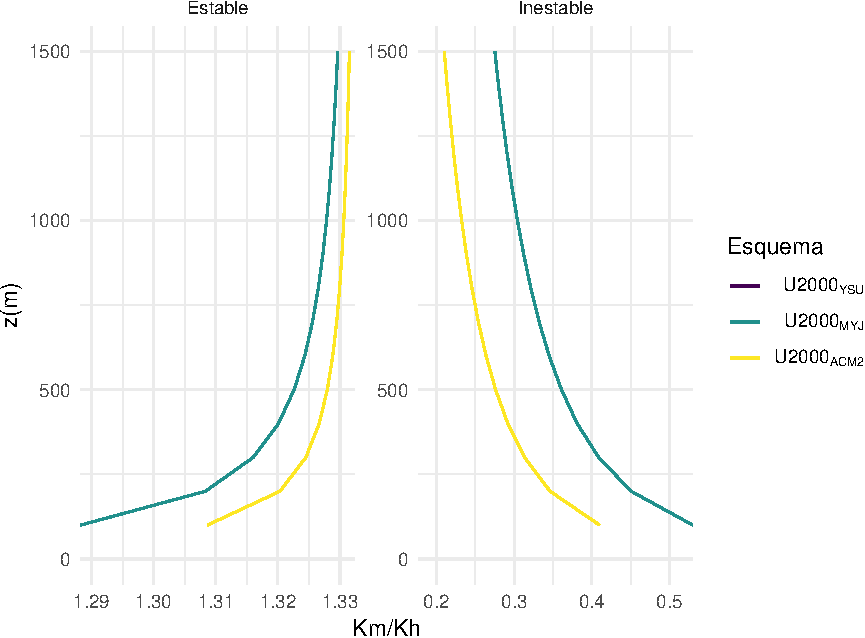
\includegraphics{00_Paper_files/figure-latex/pr-1} 

}

\caption{Variación del número de Prandtl calculado a partir del modelo propuesto por Ulke 2000 con las variables de cada simulación y promediado en cada periodo. \label{Pr}}\label{fig:pr}
\end{figure}

\begin{table}

\caption{\label{tab:tabla-clp}Parámetros característicos de la capa límite para cada simulación y regimen, promediados para todo el periodo y todo el perfil (en los casos que corresponda). \label{tabla-clp}}
\centering
\begin{tabular}[t]{llrrrrr}
\toprule
Simulación & Regimen & $\overline{h}$\textsuperscript{1} & $\overline{L}$\textsuperscript{2} & $\overline{u*}$\textsuperscript{3} & $\overline{Pr}$\textsuperscript{4} & $h/L$\\
\midrule
YSU & Estable & 365.11 & 56.95 & 0.3094 & 1.33 & 6.41\\
YSU & Inestable & 1631.19 & -29.11 & 0.5695 & 0.24 & -56.03\\
MYJ & Estable & 443.26 & 116.74 & 0.3298 & 1.33 & 3.80\\
MYJ & Inestable & 1553.56 & -80.52 & 0.5822 & 0.31 & -19.29\\
ACM2 & Estable & 200.24 & 56.95 & 0.2812 & 1.33 & 3.52\\
ACM2 & Inestable & 1944.48 & -29.11 & 0.5921 & 0.24 & -66.79\\
\bottomrule
\multicolumn{7}{l}{\textsuperscript{1} Altura de la CLP promediada.}\\
\multicolumn{7}{l}{\textsuperscript{2} Longitud de Monin Obukhov promediada.}\\
\multicolumn{7}{l}{\textsuperscript{3} Velocidad de fricción promediada.}\\
\multicolumn{7}{l}{\textsuperscript{4} Número de Prandtl promediado.}\\
\end{tabular}
\end{table}

\begin{figure}

{\centering \subfloat[Calor $K_h$ ($m^2/s$). \label{kh-wrf}\label{fig:k_ulke_wrf1}]{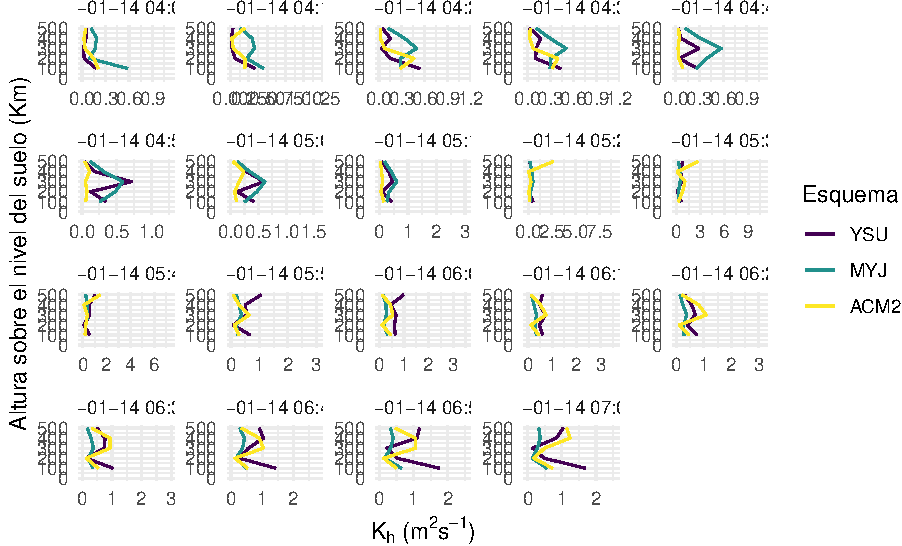
\includegraphics{00_Paper_files/figure-latex/k_ulke_wrf-1} }\newline\subfloat[Moviento $K_m$ ($m^2/s$). \label{km-wrf}\label{fig:k_ulke_wrf2}]{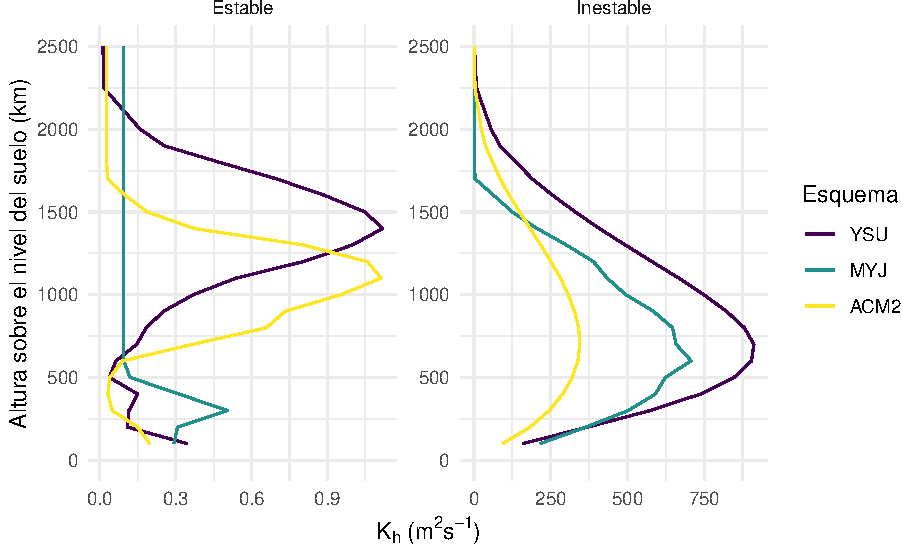
\includegraphics{00_Paper_files/figure-latex/k_ulke_wrf-2} }\newline\subfloat[Calor $K_h$ ($m^2/s$). \label{kh-wrf}\label{fig:k_ulke_wrf3}]{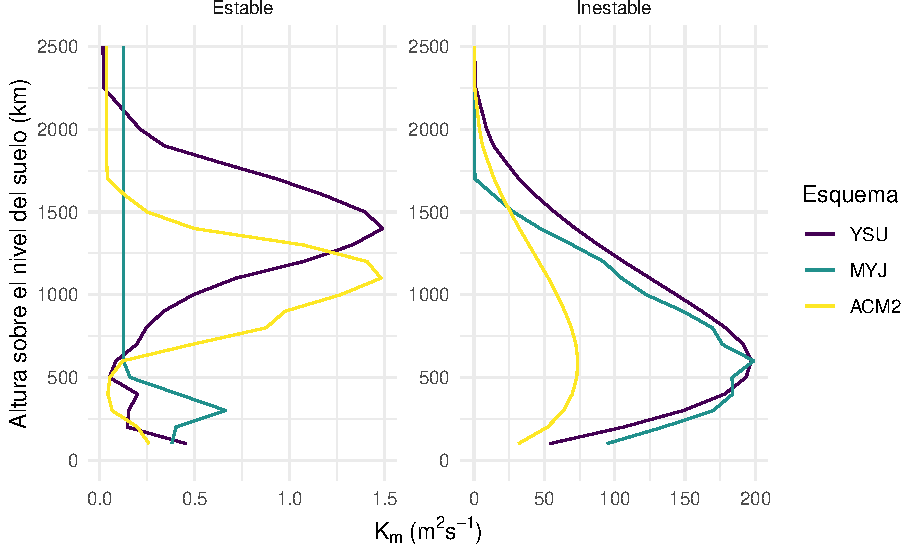
\includegraphics{00_Paper_files/figure-latex/k_ulke_wrf-3} }

}

\caption{Coeficientes de difusividad turbulenta de calor sensible (a) y cantidad de movimiento (b) promediados entre las 05 y 06 UTC (período estable, izquierda) y entre las 16 y 17 UTC (período inestable, derecha) de la capa límite en todas las simulaciones.  \label{k-ulke-wrf}}\label{fig:k_ulke_wrf}
\end{figure}

\hypertarget{refs}{}
\hypertarget{ref-Amante2009}{}
Amante, C., y Eakins, B., 2009. ETOPO1 1 Arc-Minute Global Relief Model:
Procedures, Data Sources and Analysis.

\hypertarget{ref-Kalnay1996}{}
Kalnay, E., Kanamitsu, M., Kistler, R., Collins, W., Deaven, D., Gandin,
L., Iredell, M., Saha, S., White, G., y Woollen, J. y otros, 1996. The
NCEP/NCAR 40-Year Reanaysis Project. Bulletin of the American
Meteorological Society, 77, 3, 437-471.


\end{document}
